\section{Constructing the Pinhole Camera Model}

\subsection{Nomenclature}
\begin{figure}[H]
    \centering
    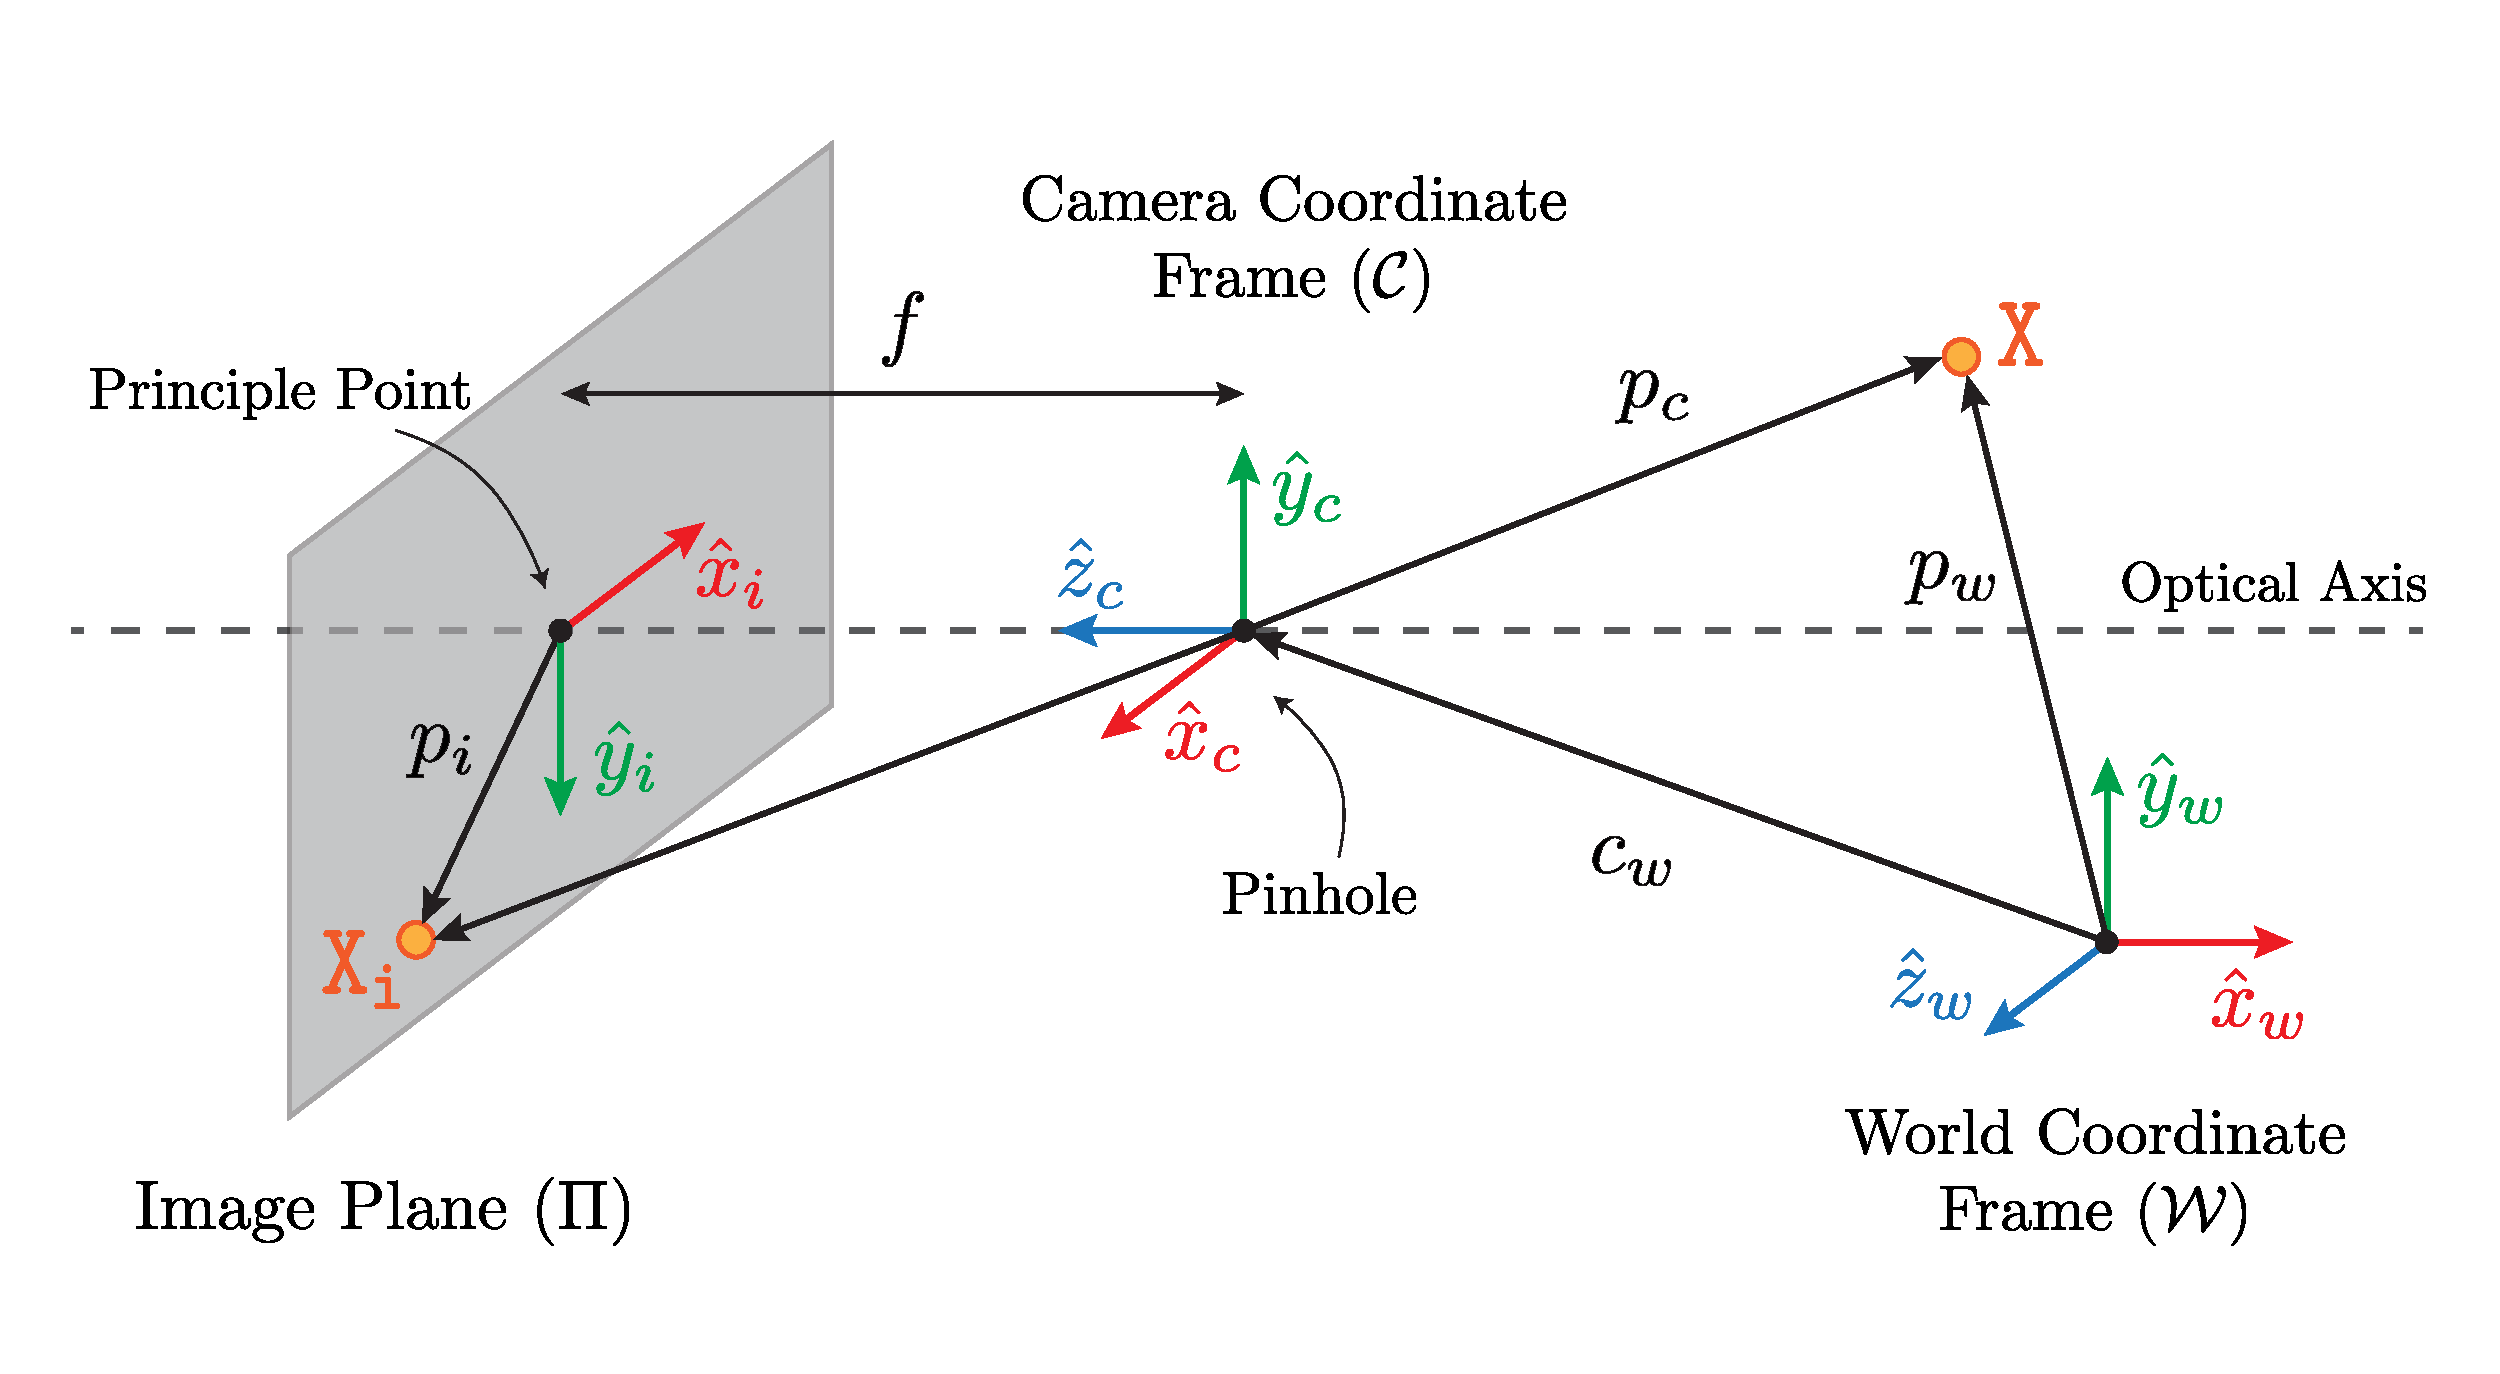
\includegraphics[width=0.9\textwidth]{figures/imaging_model}
    \caption{Pinhole camera model.}
\end{figure}

For our camera model, we will introduce 4 different coordinate systems:
\begin{itemize}[leftmargin=!, itemindent=-4ex]
    \item\textbf{The World Coordinate Frame $\boldsymbol{\mathcal{W}}$}. Points are denoted as $\left(x_w, y_w, z_w\right)$
    \item\textbf{The Camera Coordinate Frame $\boldsymbol{\mathcal{C}}$}. Points are denoted as $\left(x_c, y_c, z_c\right)$.
    \item\textbf{The Image Plane $\boldsymbol{\Pi}$}. Points are denoted as $\left(x_i, y_i\right)$.
    \item\textbf{The Sensor Grid}. Points are denoted as $\left(u, v\right)$.
\end{itemize}




\begin{figure}[H]
    \centering
    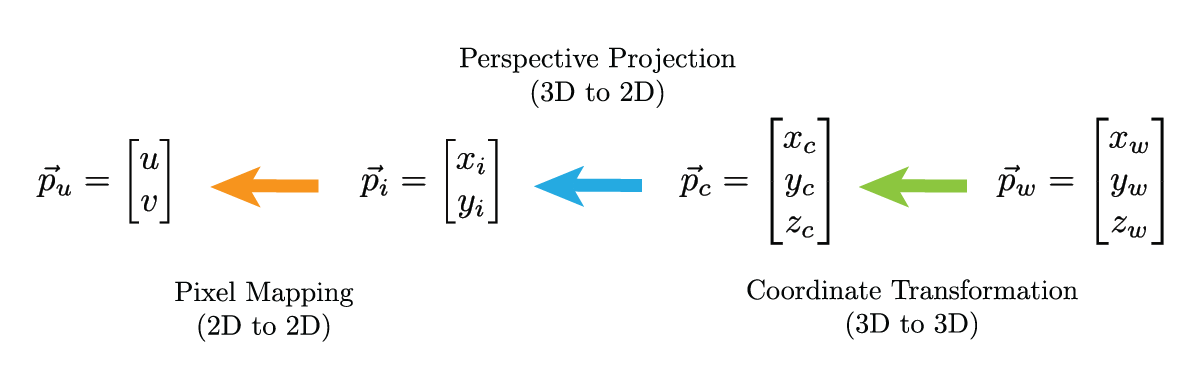
\includegraphics[width=0.9\textwidth]{figures/coord_conversions}
    \caption{Coordinate transformations.}
\end{figure}


\subsection{Intrinsic Parameters} \label{sec:intrinsics}

First, we will focus on the projection of points in the 3D space onto the image plane. The goal is to construct a calibration matrix, $K$, which relates the position of the point $P$ to its projection on the image plane. This can be expressed mathematically as follows:
\begin{equation} \label{eq:pi}
    \widetilde{p}_i =  K\widetilde{p}_c
\end{equation}
where $\vec{p}_i$ and $\vec{p}_c$ represents the position of the point $P$ in the image plane $\Pi$ and the camera frame $\mathcal{C}$ respectively.
\begin{figure}[H]
    \centering
    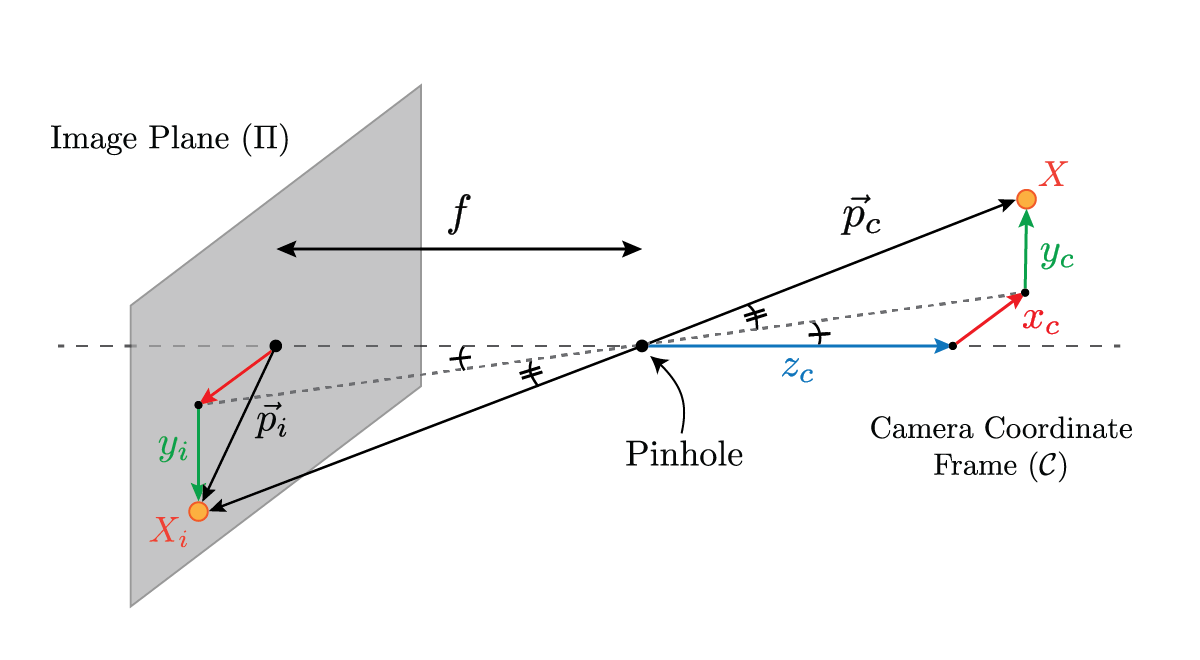
\includegraphics[width=0.9\textwidth]{figures/perspective_projection}
    \caption{Perspective projection of the point $P$ onto the image plane $\Pi$.}
\end{figure}
When a straight line is drawn from $P$ to its projection $P_i$ through the aperture, it intersects the optical axis. Deconstructing this intersection in the $x$ and $y$ direction, pairs of similar triangles are formed on the $x$ and $y$ plane.
\begin{figure}[H]
    \centering
    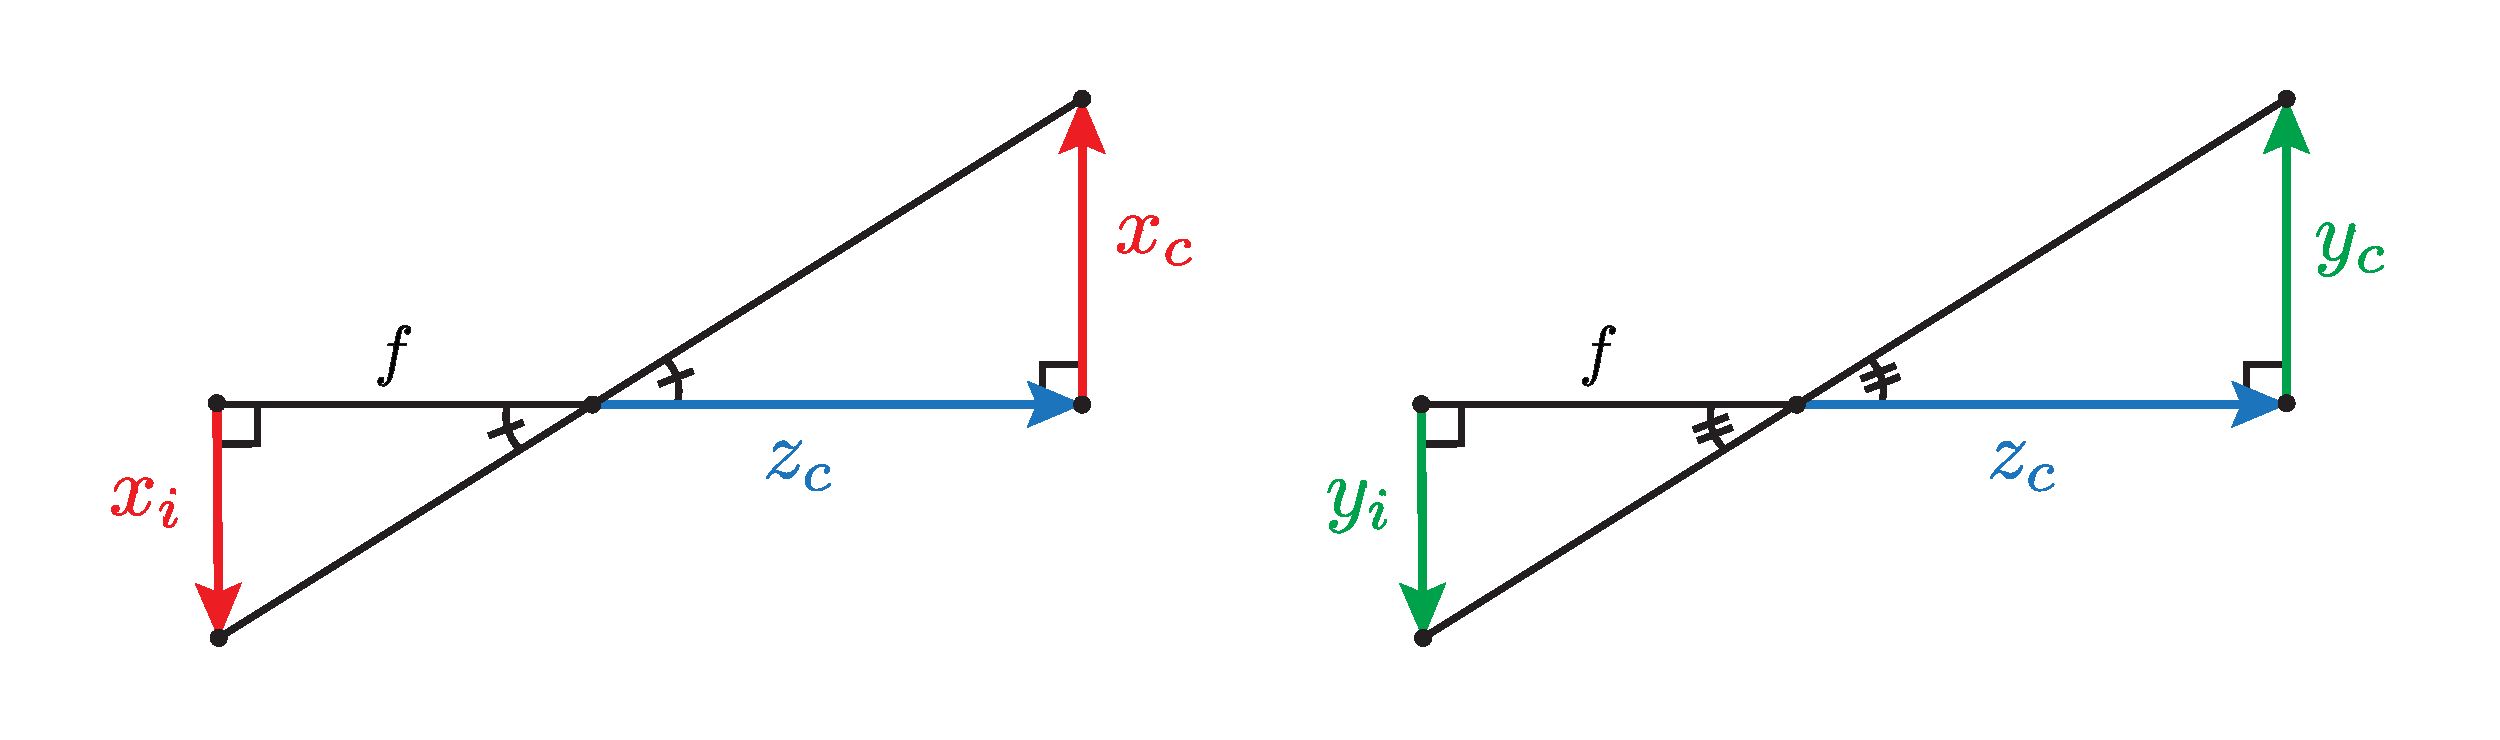
\includegraphics[width=\textwidth]{figures/similar_triangles}
    \caption{Similar triangles formed by perspective projection, which relate $x_i$ to $x_c$ and $y_i$ to $y_c$.} \label{fig:similar_triangles}
\end{figure}
\begin{subequations}
    \begin{gather}
        \frac{x_i}{f} = \frac{x_c}{z_c} \quad \Longrightarrow \quad x_i = f \frac{x_c}{z_c} \label{subeq:xi_result}\\
        \frac{y_i}{f} = \frac{y_c}{z_c} \quad \Longrightarrow \quad y_i = f \frac{y_c}{z_c} \label{subeq:yi_result}
    \end{gather}
\end{subequations}
We can then relate the coordinates of the projection, $(x_i, y_i)$, which are in real-world units, to its position $(u, v)$ in pixels.
\begin{figure}[H]
    \centering
    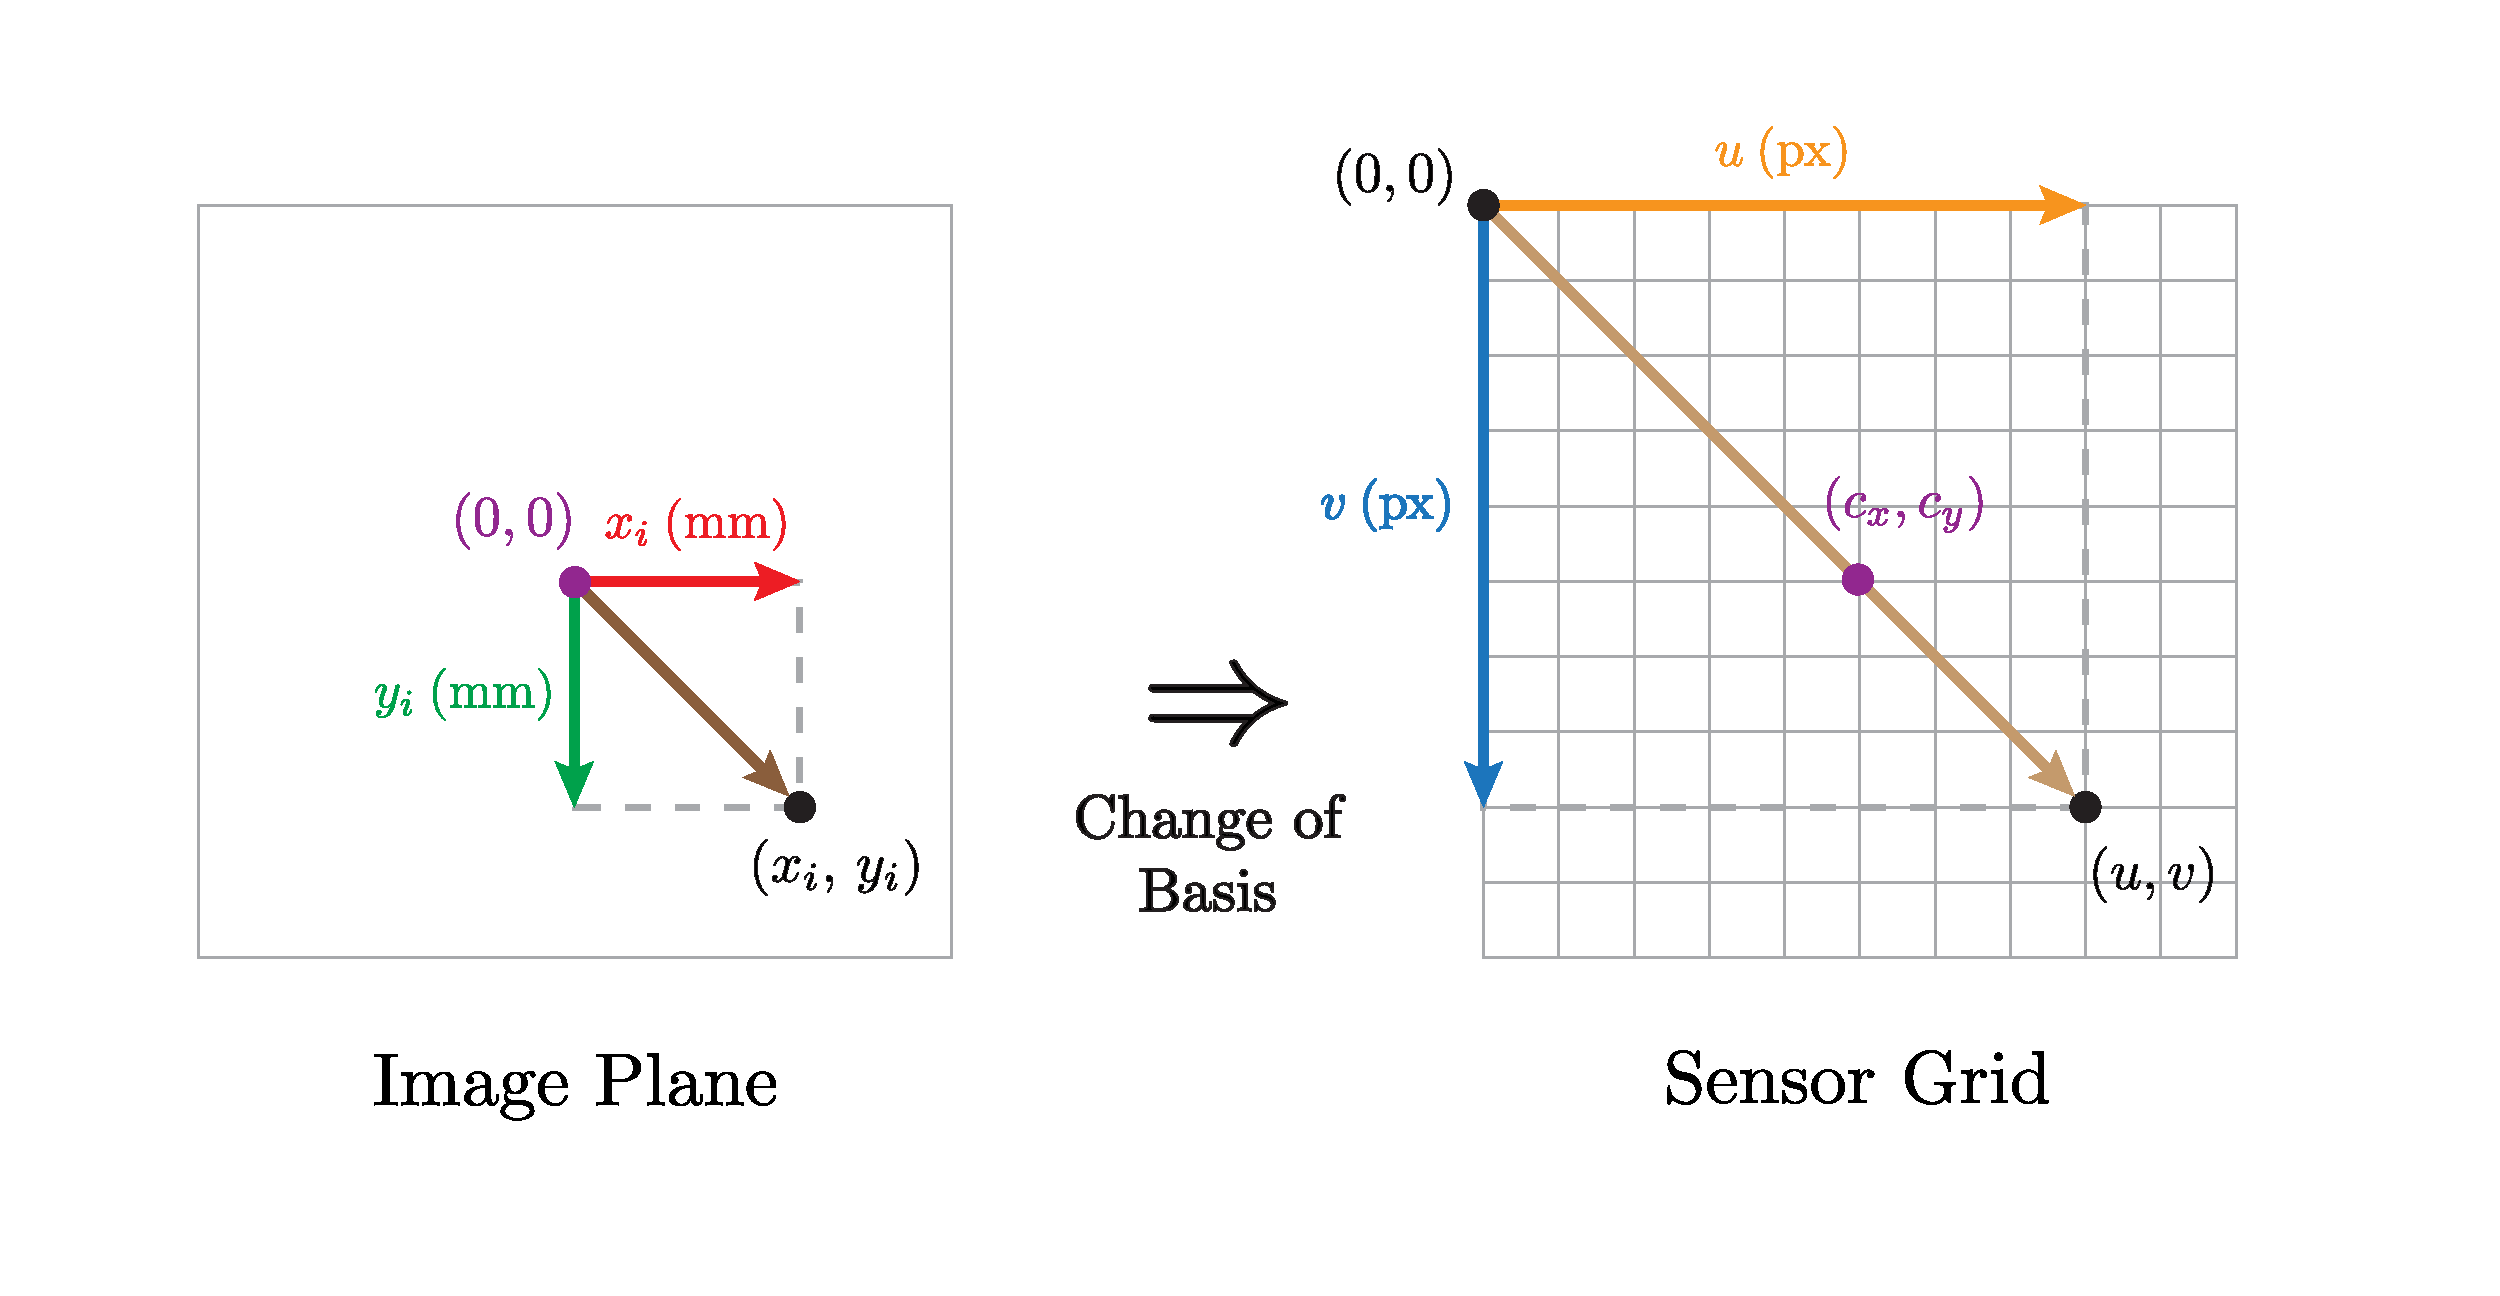
\includegraphics[width=\textwidth]{figures/sensor_grid}
    \caption{Conversion from image plane coordinates to sensor grid coordinates}
\end{figure}
Let $m_x$ and $m_y$ represent the pixel density of the image sensor in the $x$ and $y$ axes of the image sensor plane respectively.
\begin{align*}
    u = m_x x_i + c_x \\
    v = m_y y_i + c_y
\end{align*}
Replacing $x_i$ and $y_i$ for the result we obtained from \ref{subeq:xi_result} and \ref{subeq:yi_result}, we get:
\begin{align*}
    u = m_x f \frac{x_c}{z_c} + c_x \\
    v = m_y f \frac{y_c}{z_c} + c_y
\end{align*}
Since $m_x$, $m_y$, and $f$ are all unknowns, we can combine the products $m_x f$ and $m_y f$ to $f_x$ and $f_y$ respectively. Under this new scheme, we define $f_x$ and $f_y$ as the horizontal and vertical focal lengths of camera.
\begin{gather*}
    u = f_x \frac{x_c}{z_c} + c_x \\
    v = f_y \frac{y_c}{z_c} + c_y
\end{gather*}
Multiply both sides of the equations by $z_c$.
\begin{subequations}
    \begin{gather}
        z_c u = f_x x_c + z_c c_x \\
        z_c v = f_y y_c + z_c c_y
    \end{gather}
\end{subequations}
Doing so allows us to express the relationship as a matrix transformation using homogenous coordinates, by letting $\widetilde{w} = z_c$. 
\begin{equation}
    \begin{bmatrix}
        z_c u \\ z_c v \\ z_c
    \end{bmatrix}
    =
    \begin{bmatrix}
        f_x x_c + z_c c_x \\ f_y y_c + z_c c_y \\ z_c
    \end{bmatrix}
    =
    \underbrace{
        \begin{bmatrix}
            f_x & 0   & c_x \\
            0   & f_y & c_y \\
            0   & 0   & 1
        \end{bmatrix}
    }_{\mathlarger{K}}
    \begin{bmatrix}
        x_c \\ y_c \\ z_c
    \end{bmatrix}
\end{equation}

\begin{equation}
    K =
    \begin{bmatrix}
        f_x & 0   & c_x \\
        0   & f_y & c_y \\
        0   & 0   & 1
    \end{bmatrix}
\end{equation}
In this case, $K$ is what is known as the \emph{calibration matrix}. It is a matrix transformation which maps a point represented in the camera coordinate frame to the coordinates of their projection onto the sensor plane. An important property worth noting is that $K$ is an \emph{upper triangular matrix}. It is a special kind of square matrix with all of its non-zero entries above the main diagonal. This is an important property which we will exploit when extracting the intrinsic matrix from the projection matrix in section \ref{sec:projection}.

\subsection{Extrinsic Parameters} \label{sec:extrinsics}

Next, we need to establish the relationship between position of a point in the camera coordinate frame $\mathcal{C}$ to their position in the world coordinate frame $\mathcal{W}$. To do so, we find the extrinsic matrix, $M_{ext}$, which relates the positional vector $\vec{p}_w$ of point $P$ in $\mathcal{W}$, to its positional vector $\vec{p}_c$ in $\mathcal{C}$. Similar to what we did in section \ref{sec:intrinsics}, we can express this in homogenous coordinates as follows:
\begin{equation} \label{eq:pc}
    \widetilde{p}_c =  M_{ext}\,\widetilde{p}_w
\end{equation}

\begin{figure}[H]
    \centering
    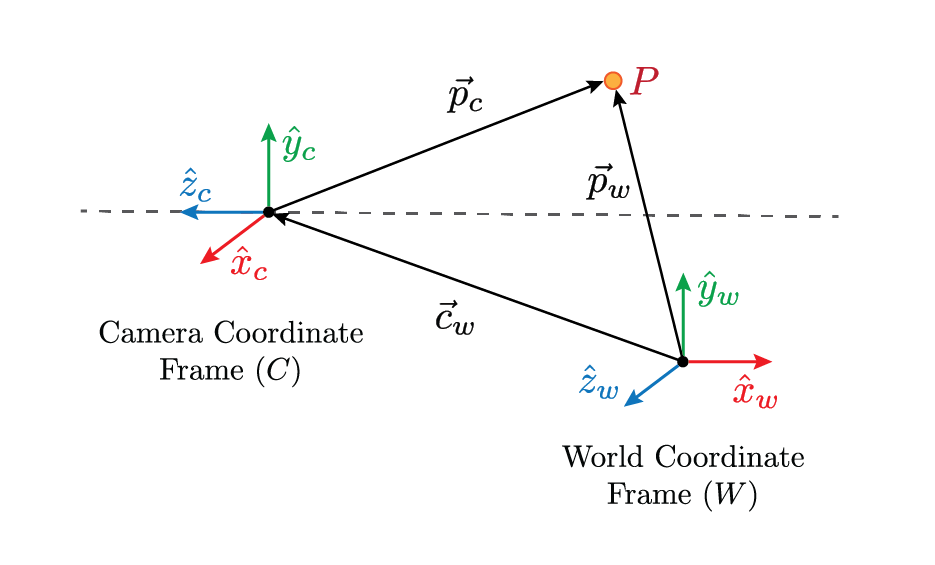
\includegraphics[width=0.9\textwidth]{figures/coord_transform}
    \caption{Coordinate transformation from the world coordinate frame to the camera frame.}
\end{figure}


For the extrinsic parameters of the camera, we have the position $\vec{c}_w$ of the camera in world coordinates and orientation $R$ of the camera. The orientation, $R$, is a 3x3 rotational matrix:

\begin{equation}
    R =
    \begin{bmatrix}
        r_{11} & r_{12} & r_{13} \\
        r_{21} & r_{22} & r_{23} \\
        r_{31} & r_{32} & r_{33}
    \end{bmatrix}
\end{equation}

\noindent where:
\begin{itemize}
    \item Row 1: Direction of $\hat{x}_c$ in world coordinate frame.
    \item Row 2: Direction of $\hat{y}_c$ in world coordinate frame.
    \item Row 3: Direction of $\hat{z}_c$ in world coordinate frame.
\end{itemize}

\noindent

\begin{subequations}
    \begin{align}
        \vec{p}_c & = R(\vec{p}_w-\vec{c}_w) \\
                  & = R\vec{p}_w -R\vec{c}_w
    \end{align}
\end{subequations}



\begin{gather}
    \vec{p}_c = R\vec{p}_w + \vec{t} \\
    \begin{bmatrix}
        x_c \\ y_c \\ z_c
    \end{bmatrix}
    =
    \underbrace{
        \begin{bmatrix}
            r_{11} & r_{12} & r_{13} \\
            r_{21} & r_{22} & r_{23} \\
            r_{31} & r_{32} & r_{33}
        \end{bmatrix}
    }_{\mathlarger{R}}
    \begin{bmatrix}
        x_w \\ y_w \\ z_w
    \end{bmatrix}
    +
    \underbrace{
        \begin{bmatrix}
            t_x \\ t_y \\ t_z
        \end{bmatrix}
    }_{\mathlarger{\vec{t}}}
\end{gather}


\begin{equation}
    \begin{bmatrix}
        x_c \\ y_c \\ z_c \\ 1
    \end{bmatrix}
    =
    \underbrace{
        \begin{bmatrix}
            r_{11} & r_{12} & r_{13} & t_x \\
            r_{21} & r_{22} & r_{23} & t_y \\
            r_{31} & r_{32} & r_{33} & t_z \\
            0      & 0      & 0      & 1
        \end{bmatrix}
    }_{\mathlarger{M_{ext}}}
    \begin{bmatrix}
        x_w \\ y_w \\ z_w \\1
    \end{bmatrix}
\end{equation}

\begin{equation}
    M_{ext} =
    \begin{bmatrix}
        R & t \\
        0 & 1
    \end{bmatrix}
\end{equation}

